\section{Architecture}
\label{sec:archi}
Let's look at the general user scenario of PredicTV recommender system.
The user first upgrades his or her Internet-enabled TV set-top box by
installing the PredicTV client-side firmware.
This firmware allows the set-top box to capture every channel switching
action while the user is watching TV by recording the time of the switch
and the new channel the user switches to. Then in real time, the set-top
box, acting as a PredicTV client, streams the channel switching records over
the Internet to the PredicTV server. This information serves as the
dynamic viewing behavior of the user(s) for this particular set-top box.
From the timings and the channels of two consecutive switches,
the system can infer which programs the user has watched and for how long.
And these values are the basis for modeling the users' watching preferences.
PredicTV server interacts with many such TV set-top boxes at the same time
and maintains a user model for each box. In addition to sending the
channel switching updates, the client can also query the server for
recommendation on user-demand or regular basis. Whenever the system receives
such a query, it looks at the current preference model of the user,
selects one or more most suitable programs to be aired in the near future,
and notifies the user of these choices.

\begin{figure}[h]
\begin{center}
\epsfig{file=archi.eps,width=\columnwidth}
\caption{PredicTV System Architecture}
\label{fig:archi}
\end{center}
\end{figure}

As depicted in Figure \ref{fig:archi}, the PredicTV server
can be divided into three basic components: communication module,
web information extraction module, and recommendation module.
Of these, the web information module and the reccommendation module
form the core recommendation engine and will be discussed in
detail in Section \ref{sec:algo}. Here we focus more on the communication
module.

Communication module is responsible for the interaction between the
client and the server. It retrieves users' channel switch
updates or recommendation requests from a work queue and forwards them to the
recommendation module. When a recommendation is made, the worker returns
the results to the communication module.
%{\bf Zhiyuan to rewrite this para.}

The communication module uses XML to pass messages.
Figure \ref{fig:xml} shows an
example of message of a channel-switch action.

\begin{figure}[h]
\begin{center}
%\begin{minipage}[c]{\columnwidth}
%\fbox{
\small
\begin{Verbatim}[frame=single]
<?xml version="1.0" enconding="utf-8 ?">
<msn>
  <command type="switch-ch"
    time="20110501-12:04:05"
    user="predictvuser123@hotmail.com">
    <item serviceid="201"
      time="20100501-12:04:04"
      duration=600>
  </command>
</msn>
\end{Verbatim}
%}
%}
%\end{minipage}
\caption{\label{fig:xml}Channal-Switching Message}
\end{center}
\end{figure}

In this message, ``Type'' attribute in {\tt command} tag describes
the interaction type with user. Action type {\tt switch-ch} means user is
switching to a new channel. {\tt Item} tag is used to describe the
previous channel user watches. {\tt Duration} attribute stands for the
time user stays in that channel, with second as the unit.
%======= Move following to algo ====================

Recommendation module is the core of our system. It uses users' viewing
behaviour information as the
input of its analysis process then replies recommendation results to users
via Communication module. Since in mainland China, we don't have standard
and detailed TV program information available, we have to obtain such
information ourself. That's why Information Extraction module is involved
in our system. It grabs HTML files from the internet, filters unnecessary
parts, then passes them to recommendation module. Database module is
basically a database service. We implements some database access
interfaces so that other modules can use the database more easily.

The Information Extraction module has two tasks. One is to grab HTML files
from the internet, another is to remove trivial information from files we
grab. We use Baidu and Google to finish the first task. For a program
that we want to collect its information, we form an URL based on Baidu
and Google's rules. Then we send HTTP requests to both these two sites
and get replies. Baidu and Google will reply the URLs of websites most fit
the key word we provide, so we send HTTP requests again and get HTML files
we need. Though Baidu and Google help us to search the websites most
related to our key words, there will still be some noise in the HTML files,
basically a database service. We implements some database access
interfaces so that other modules can use the database more easily.
